%
% Modified by Megan Patnott
% Last Change: Jan 18, 2013
%
%%%%%%%%%%%%%%%%%%%%%%%%%%%%%%%%%%%%%%%%%%%%%%%%%%%%%%%%%%%%%%%%%%%%%%%%
%
% Modified by Sameer Vijay
% Last Change: Wed Jul 27 2005 13:00 CEST
%
%%%%%%%%%%%%%%%%%%%%%%%%%%%%%%%%%%%%%%%%%%%%%%%%%%%%%%%%%%%%%%%%%%%%%%%%
%
% Sample Notre Dame Thesis/Dissertation
% Using Donald Peterson's ndthesis classfile
%
% Written by Jeff Squyres and Don Peterson
%
% Provided by the Information Technology Committee of
%   the Graduate Student Union
%   http://www.gsu.nd.edu/
%
% Nothing in this document is serious except the format.  :-)
%
% If you have any suggestions, comments, questions, please send e-mail
% to: ndthesis@gsu.nd.edu
%
%%%%%%%%%%%%%%%%%%%%%%%%%%%%%%%%%%%%%%%%%%%%%%%%%%%%%%%%%%%%%%%%%%%%%%%%

%
% Chapter 4
%


\chapter{DIELECTRIC PROPERTIES}
\label{chap:dielectric}
In the previous chapter, we have derived various physical properties considering SP, GSF, and TSF methods and tested result against the multipolar Ewald method. In this chapter, we discuss fluctuation, perturbation, and potential of mean force (PMF) methods for calculating the dielectric properties of the dipolar and quadrupolar fluids using newly developed real space methods. Since the dielectric constant is a macroscopic property, the interactions of a molecule with the rest of the molecules of the system are important. Our newly developed real space methods utilize a cutoff radius which reduces the number of interactions calculated in the system. Hence, the formula for the dielectric constant should be modified accordingly. Therefore to get correct dielectric properties using the result obtained from the simulation, we need to evaluate correction factor for each real-space methods separately. In this chapter, we have also calculated the correction factors for each real-space methods and tabulated for both dipolar and quadrupolar fluids.

\section{Introduction}
One of the most difficult tests of any new electrostatic method is the
fidelity with which that method can reproduce the bulk-phase
polarizability or equivalently, the dielectric properties of a
fluid. Before the advent of computer simulations, Kirkwood and Onsager
developed fluctuation formulae for the dielectric properties of
dipolar fluids.\cite{Kirkwood39,Onsagar36}
Of particular interest is the static dielectric constant, $\epsilon$.
Using the Ewald sum under tin-foil boundary conditions, $\epsilon$ can
be calculated for systems of non-polarizable substances via
\begin{equation}
\epsilon = 1 + \frac{\langle M^2\rangle}{3\epsilon_0k_\textrm{B}TV},
\label{eq:staticDielectric}
\end{equation}
where $\epsilon_0$ is the permittivity of free space and
$\langle M^2\rangle$ is the fluctuation of the system dipole
moment.\cite{Allen89} The numerator in the fractional term in
equation (\ref{eq:staticDielectric}) is identical to the quantity
calculated in the finite-system Kirkwood $g$ factor ($G_k$):
\begin{equation}
G_k = \frac{\langle M^2\rangle}{N\mu^2},
\label{eq:KirkwoodFactor}
\end{equation}
where $\mu$ is the dipole moment of a single molecule of the
homogeneous system.\cite{NeumannI83,NeumannII83,Neumann84,Neumann85} The
fluctuation term in both equation (\ref{eq:staticDielectric}) and
(\ref{eq:KirkwoodFactor}) is calculated as follows,
\begin{equation}
\begin{split}
\langle M^2\rangle &= \langle\bm{M}\cdot\bm{M}\rangle 
                        - \langle\bm{M}\rangle\cdot\langle\bm{M}\rangle \\
                   &= \langle M_x^2+M_y^2+M_z^2\rangle
                        - (\langle M_x\rangle^2 + \langle M_x\rangle^2 
                                + \langle M_x\rangle^2).        
\end{split}
\label{eq:fluctBoxDipole}
\end{equation}
This fluctuation term can be accumulated during a simulation; however,
it converges rather slowly, thus requiring multi-nanosecond simulation
times.\cite{Horn04} In the case of tin-foil boundary conditions, the
dielectric/surface term of the Ewald summation is equal to zero.

Similar formulae were developed by Logan \textit{et al.} for the bulk
polarizability of quadrupolar fluids.\cite{LoganI81,LoganII82,LoganIII82}
In modern simulations, bulk materials are usually treated using
periodic replicas of small regions, and this level of approximation
requires corrections to the fluctuation formulae that were derived for
the bulk fluids. In 1983 Neumann proposed a general formula for
evaluating dielectric properties of dipolar fluids using real-space
cutoff methods.\cite{NeumannI83} Steinhauser and Neumann used this
formula to evaluate the corrected dielectric constant for the
Stockmayer fluid using two different methods: Ewald-Kornfield (EK) and
reaction field (RF) methods.\cite{NeumannII83}

Zahn \textit{et al.}\cite{Zahn02} utilized this approach and evaluated
the correction factor for using damped shifted charge-charge
kernel. This was later generalized by Izvekov \textit{et
  al.},\cite{Izvekov08} who that the expression for the
dielectric constant reduces to widely-used \textit{conducting
  boundary} formula for real-space cutoff methods that have first
derivatives that vanish at the cutoff sphere.

In quadrupolar fluids, the relationship between quadrupolar
susceptibility and the dielectric constant is not as straightforward
as in the dipolar case. The dielectric constant depends on the
geometry of the external field perturbation.\cite{Ernst92} Significant
efforts have been made to increase our understanding the dielectric
properties of these fluids,\cite{JeonI03,JeonII03,Chitanvis96}
although a correction formula for different real-space methods has not
yet been developed.

In this paper we derive general formulae for calculating the
dielectric properties of quadrupolar fluids. We also evaluate the
correction factor for SP, GSF, and TSF methods for both dipolar and
quadrupolar fluids interacting via point charges, point dipoles or
through quadrupole-quadrupole interactions.

We have also calculated the screening behavior for two ions immersed
in a quadrupolar fluid to estimate the dielectric screening from the
quadrupolar susceptibility.  We have used three different methods to
compare our results with computer simulations:
\begin{enumerate}
\item responses of the fluid to external perturbations,
\item fluctuations of box multipole moments, and
\item potentials of mean force between solvated ions,
\end{enumerate}

In the external field perturbation, the net polarization of the system
is observed as a linear response of the applied field perturbation,
where proportionality constant is determined by the electrostatic
interaction between the electrostatic multipoles at a given
temperature. The fluctuation formula observes the time average
fluctuation of the multipolar moment as a function of temperature. The
average fluctuation value of the system is determined by the
multipole-multipole interactions between molecules at a given
temperature. Since the expression of the electrostatic interaction
energy, force, and torque in the real space electrostatic methods are
different from their original definition, both fluctuation and
external field perturbation formula should also be modified
accordingly. The potential of mean force method calculates dielectric
constant or screening factor from the potential energy between ions before and after dielectric material is introduced. All of these different methods for
calculating dielectric properties will be discussed in detail in the
following sections: \ref{subsec:perturbation},\ref{subsec:fluctuation}, and \ref{sec:PMF}.

\section{Boltzmann average for orientational polarization}
The dielectric properties of the system is mainly arise from two different ways: i) the applied field distort the charge distributions so it produces an induced multipolar moment in each molecule; and ii) the applied field tends to line up originally randomly oriented molecular moment towards the direction of the applied field. In this study, we basically focus on the orientational contribution in the dielectric properties. If we consider a system of molecules in the presence of external field perturbation, the perturbation experienced by any molecule will not be only due to external field or field gradient but also due to the field or field gradient produced by the all other molecules in the system. In the following subsections \ref{subsec:boltzAverage-Dipole} and \ref{subsec:boltzAverage-Quad}, we will discuss about the molecular polarization only due to external field perturbation. The contribution of the field or field gradient due to all other molecules will be taken into account while calculating correction factor in the section \ref{sec:corrFactor}.

\subsection{Dipole}
\label{subsec:boltzAverage-Dipole}
Consider a system of molecules, each with permanent dipole moment
$p_o$. In the absense of external field, thermal agitation orients the
dipoles randomly, reducing the system moment to zero.  External fields
will tend to line up the dipoles in the direction of applied field.
Here we have considered net field from all other molecules is
considered to be zero.  Therefore the total Hamiltonian of each
molecule is,\cite{Jackson98}
\begin{equation}
H = H_o - \bf{p_o} .\bf{E},
\end{equation}
where $H_o$ is a function of the internal coordinates of the molecule.
The Boltzmann average of the dipole moment is given by,
\begin{equation}
\braket{p_{mol}} = \frac{\displaystyle\int d\Omega\; p_o\; cos\theta\;  e^{\frac{p_oE\; cos\theta}{k_B T}}}{\displaystyle\int d\Omega\; e^{\frac{p_oE\;cos\theta}{k_B T}}},
\end{equation}
where $\bf{E}$ is selected along z-axis. If we consider that the
applied field is small, \textit{i.e.} $\frac{p_oE\; cos\theta}{k_B T} << 1$, 
\begin{equation}
\braket{p_{mol}}  \approx \frac{1}{3}\frac{{p_o}^2}{k_B T}E,
\end{equation}
where $ \alpha_p = \frac{1}{3}\frac{{p_o}^2}{k_B T}$ is a molecular
polarizability. The orientational polarization depends inversely on
the temperature and applied field must overcome the thermal agitation.

\subsection{Quadrupole}
\label{subsec:boltzAverage-Quad}
Consider a system of molecules with permanent quadrupole moment $q_{\alpha\beta} $. The average quadrupole moment at temperature T in the presence of uniform applied field gradient is given by,\cite{AduGyamfi78, AduGyamfi81}
\begin{equation}
\braket{q_{\alpha\beta}} \;=\; \frac{\displaystyle\int d\Omega\; e^{-\frac{H}{k_B T}}q_{\alpha\beta}}{\displaystyle\int d\Omega\; e^{-\frac{H}{k_B T}}} \;=\; \frac{\displaystyle\int d\Omega\; e^{\frac{q_{\mu\nu}\;\partial_\nu E_\mu}{k_B T}}q_{\alpha\beta}}{\displaystyle\int d\Omega\; e^{\frac{q_{\mu\nu}\;\partial_\nu E_\mu}{k_B T}}},
\label{boltzQuad}
\end{equation}
where $\int d\Omega = \int_0^{2\pi} \int_0^\pi \int_0^{2\pi}
sin\theta\; d\theta\ d\phi\ d\psi$ is the integration over Euler
angles, $ H = H_o -q_{\mu\nu}\;\partial_\nu E_\mu $ is the energy of
a quadrupole in the gradient of the  
applied field and $ H_o$ is a function of internal coordinates of the molecule. The energy and quadrupole moment can be transformed into body frame using following relation, 
\begin{equation}
\begin{split}
&q_{\alpha\beta} = \eta_{\alpha\alpha'}\;\eta_{\beta\beta'}\;{q}^* _{\alpha'\beta'} \\
&H = H_o - q:\vec{\nabla}\vec{E} = H_o - q_{\mu\nu}\;\partial_\nu E_\mu = H_o -\eta_{\mu\mu'}\;\eta_{\nu\nu'}\;{q}^*_{\mu'\nu'}\;\partial_\nu E_\mu.
\end{split}
\label{energyQuad}
\end{equation}
Here the starred tensors are the components in the body fixed
frame. Substituting equation (\ref{energyQuad}) in the equation (\ref{boltzQuad})
and taking linear terms in the expansion we get,
\begin{equation}
\braket{q_{\alpha\beta}} = \frac{ \int d\Omega \left(1 + \frac{\eta_{\mu\mu'}\;\eta_{\nu\nu'}\;{q}^*_{\mu'\nu'}\;\partial_\nu E_\mu }{k_B T}\right)q_{\alpha\beta}}{ \int d\Omega \left(1 + \frac{\eta_{\mu\mu'}\;\eta_{\nu\nu'}\;{q}^*_{\mu'\nu'}\;\partial_\nu E_\mu }{k_B T}\right)},
\end{equation}
where $\eta_{\alpha\alpha'}$ is the inverse of the rotation matrix that transforms
the body fixed co-ordinates to the space co-ordinates,
\[\eta_{\alpha\alpha'} 
= \left(\begin{array}{ccc}
cos\phi\; cos\psi - cos\theta\; sin\phi\; sin\psi & -cos\theta\; cos\psi\; sin\phi - cos\phi\; sin\psi & sin\theta\; sin\phi \\
cos\psi\; sin\phi + cos\theta\; cos\phi \; sin\psi & cos\theta\; cos\phi\; cos\psi - sin\phi\; sin\psi & -cos\phi\; sin\theta \\
sin\theta\; sin\psi & -cos\psi\; sin\theta & cos\theta
\end{array} \right).\]
Integration of 1st and 2nd terms in the denominator gives $8 \pi^2$
and $8 \pi^2 /3\;\vec{\nabla}.\vec{E}\; Tr(q^*) $ respectively. The
second term vanishes for charge free space
(i.e. $\vec{\nabla}.\vec{E} \; = \; 0)$. Similarly integration of the
1st term in the numerator produces
$8 \pi^2 /3\; Tr(q^*)\delta_{\alpha\beta}$ and the 2nd term produces
$8 \pi^2 /15k_B T (3{q}^*_{\alpha'\beta'}{q}^*_{\beta'\alpha'} -
{q}^*_{\alpha'\alpha'}{q}^*_{\beta'\beta'})\partial_\alpha E_\beta$,
if $\vec{\nabla}.\vec{E} \; = \; 0$,
$ \partial_\alpha E_\beta = \partial_\beta E_\alpha$ and
${q}^*_{\alpha'\beta'}= {q}^*_{\beta'\alpha'}$. Therefore the
Boltzmann average of a quadrupole moment can be written as,

\begin{equation}
\braket{q_{\alpha\beta}}\; = \; \frac{1}{3} Tr(q^*)\;\delta_{\alpha\beta} + \frac{{\bar{q_o}}^2}{15k_BT}\;\partial_\alpha E_\beta,
\end{equation}
where $ \alpha_q = \frac{{\bar{q_o}}^2}{15k_BT} $ is a molecular quadrupolarizablity  and  ${\bar{q_o}}^2=
3{q}^*_{\alpha'\beta'}{q}^*_{\beta'\alpha'}-{q}^*_{\alpha'\alpha'}{q}^*_{\beta'\beta'}$ is a square of the net quadrupole moment of a molecule. 

\section{Macroscopic Polarizability}
\label{sec:MacPolarizablity}

If we consider a system of dipolar or quadrupolar fluid in the external field perturbation, the net polarization of the system will still be proportional to the applied field perturbation.\cite{Chitanvis96, Stern-Feller03, SalvchovI14, SalvchovII14} In simulation the net polarization of the system is determined by the interaction of molecule with all other molecules as well as external field perturbation. Therefore the macroscopic polarizablity obtained from the simulation always varies with nature of real-space electrostatic interaction methods implemented in the simulation. To determine a susceptibility or dielectric constant of the material (which is a actual physical property of the dipolar or quadrupolar fluid) from the macroscopic polarizablity, we need to incorporate the interaction between molecules which has been discussed in detail in section \ref{sec:corrFactor}. In this section we discuss about the two different methods of calculating macroscopic polarizablity for both dipolar and quadrupolar fluid. 

\subsection{External field perturbation}
\label{subsec:perturbation}
In the presence of uniform electric field $\textbf{E}^o$, a system of dipolar  molecules polarizes along the direction of the applied field (or field gradient). Therefore the net dipolar polarization $ \textbf{P}$ of the system is,
\begin{equation}
\textbf{P} = \epsilon_o \alpha_{D}\; \textbf{E}^o. 
\label{pertDipole}
\end{equation} 
The constant $\alpha_D$ is a macroscopic polarizability, which is a property of the dipolar fluid in a given density and temperature.

Similarly, in the presence of external field gradient the system of quadrupolar molecule polarizes along the direction of applied field gradient therefore the net quadrupolar polarization of the system can be given by,
\begin{equation}
\begin{split}
& {Q}_{\alpha\beta} = \frac{1}{3}\; Tr({Q})\; \delta_{\alpha\beta} +  \epsilon_o\; \alpha_Q \; \partial_{\alpha} E^o_{\beta} 
\\ & or \\
& \frac{1}{3}\;\Theta_{\alpha\beta} =  \epsilon_o\; \alpha_Q \; \partial_{\alpha} E^o_{\beta} 
\end{split}
\label{pertQuad}
\end{equation} 
where $Q_{\alpha\beta}$ is a tensor component of the traced quadrupolar moment of the system, $ \alpha_Q$ is a macroscopic quadrupolarizability has a dimension of $length^{-2}$, and $\Theta_{\alpha\beta} = 3Q_{\alpha\beta}-Tr(Q) $ is the traceless component of the quadrupole moment.    

\subsection{Fluctuation formula}
\label{subsec:fluctuation}
For a system of molecules with net dipolar moment $\bf{M}$ at thermal equilibrium of temperature T in the presence of applied field $\bf{E}^o$, the average dipolar polarization can be expressed in terms of fluctuation of the net dipole moment as below,\cite{Stern03}
\begin{equation}
\braket{\bf{P}} = \epsilon_o \frac{\braket{\bf{M}^2}-{\braket{\bf{M}}}^2}{3 \epsilon_o V k_B T}\bf{E}^o
\label{flucDipole}
\end{equation}
This is similar to the formula for boltzmann average of single dipolar molecule in the subsection \ref{subsec:boltzAverage-Dipole}. Here $\braket{\bf{P}}$ is average polarization and $ \braket{\textbf{M}^2}-{\braket{\textbf{M}}}^2$ is the net dipole fluctuation at temperature T. For the limiting case $\textbf{E}^o \rightarrow 0 $, ensemble average of both net dipole moment $\braket{\textbf{M}}$ and dipolar polarization $\braket{\bf{P}}$ tends to vanish but $\braket{\bf{M}^2}$ will still be non-zero. The dipolar macroscopic polarizability can be written as,
\begin{equation}
\alpha_D = \frac{\braket{\bf{M}^2}-{\braket{\bf{M}}}^2}{3 \epsilon_o V k_B T}
\end{equation}
This is a macroscopic property of dipolar material which is true even if applied field $ \textbf{E}^o \rightarrow 0 $.  

Analogous formula can also be written for a system with quadrupolar molecules,
\begin{equation}
\braket{Q_{\alpha\beta}} = \frac{1}{3} Tr(\textbf{Q})\; \delta_{\alpha\beta} + \epsilon_o \frac{\braket{\textbf{Q}^2}-{\braket{\textbf{Q}}}^2}{15 \epsilon_o V k_B T}{\partial_\alpha E^o_\beta}
\label{flucQuad}
\end{equation}
where $Q_{\alpha\beta}$ is a component of system quadrupole moment,  $\bf{Q}$ is net quadrupolar moment which can be expressed as $\textbf{Q}^2 =3Q_{\alpha\beta}Q_{\alpha\beta}-(Tr\textbf{Q})^2 $. The macroscopic quadrupolarizability is given by,
\begin{equation}
\alpha_Q = \frac{\braket{\textbf{Q}^2}-{\braket{\textbf{Q}}}^2}{15 \epsilon_o V k_B T}
\label{propConstQuad}
\end{equation}

\section{Potential of mean force}
In this method, we will measure the interaction between a positive and negative charge at varying distances after introducing a dipolar (or quadrupolar) material between them. The potential of mean force (PMF) between two ions in a liquid is obtained by constraining their distance and measuring the mean constraint force required to hold them at a fixed distance $r.$ The PMF  is obtained from a sequence of simulations can be expressed as \cite{Wilfred07},
\begin{equation}
w(r) = \int_{r_o}^{r}\braket{\frac{\partial f}{\partial r'}}dr' + 2kT \log(r/r_o) + w(r_o),
\label{eq:pmf}
\end{equation}
where $\braket{\partial f/\partial r'}$ is the mean constraint force, $2kT \log(r/r_o)$ is the Fixman factor, and $r_o$ is the reference position. The potential energy between two charges at separation $r$ is given by,
\begin{equation}
w(r) = \frac{1}{4\pi\epsilon}\frac{q_1q_2}{r},
\end{equation}
where $\epsilon$ is the dielectric constant for the fluid.

The quadrupole molecule can couple with the gradient of the electric field and the two opposite point charges produces non-zero value of both electric field as well as gradient of the field. Therefore, this simulation set up can be used to determine the dielectric constant for both dipolar and quadrupolar fluid.
\label{sec:PMF}

\section{Correction factor}
\label{sec:corrFactor}
Since equations (\ref{pertDipole}, \ref{pertQuad}, \ref{flucDipole}, and \ref{flucQuad}) provide relation between polarization (dipolar or quadrupolar)  and applied field (uniform field or field gradient), $\chi_d$ (or $ \chi_q$) is actually a macroscopic polarizability (or quadrupolarizability), which is different than the dipolar (or quadrupolar) susceptibility of the fluid. Actual constitutive relation should have a relation between polarization and Maxwell field (or field gradient) at different point in the sample. We can obtain susceptibility of the fluid from its macroscopic polarizability using correction factor evaluated below.

\subsection{Dipolar system}
In the presence of an external field $ \textbf{E}$ polarization $\textbf{E}$ will be induced in a dipolar system. The total electrostatic field (or Maxwell electric field) at point $\bf{r}$ in a system is,\cite{NeumannI83}
\begin{equation}
\textbf{E}(\textbf{r}) = \textbf{E}^o(\textbf{r}) + \frac{1}{4\pi\epsilon_o} \int d^3r' \textbf{T}(\textbf{r}-\textbf{r}')\cdot {\textbf{P}(\textbf{r}')}.
\end{equation}

We can consider the cases of Stockmayer (dipolar) soft spheres that are represented either by two closely-spaced point charges or by a single point dipole (see Fig. \ref{fig:stockmayer}).
\begin{figure}
  \centering
  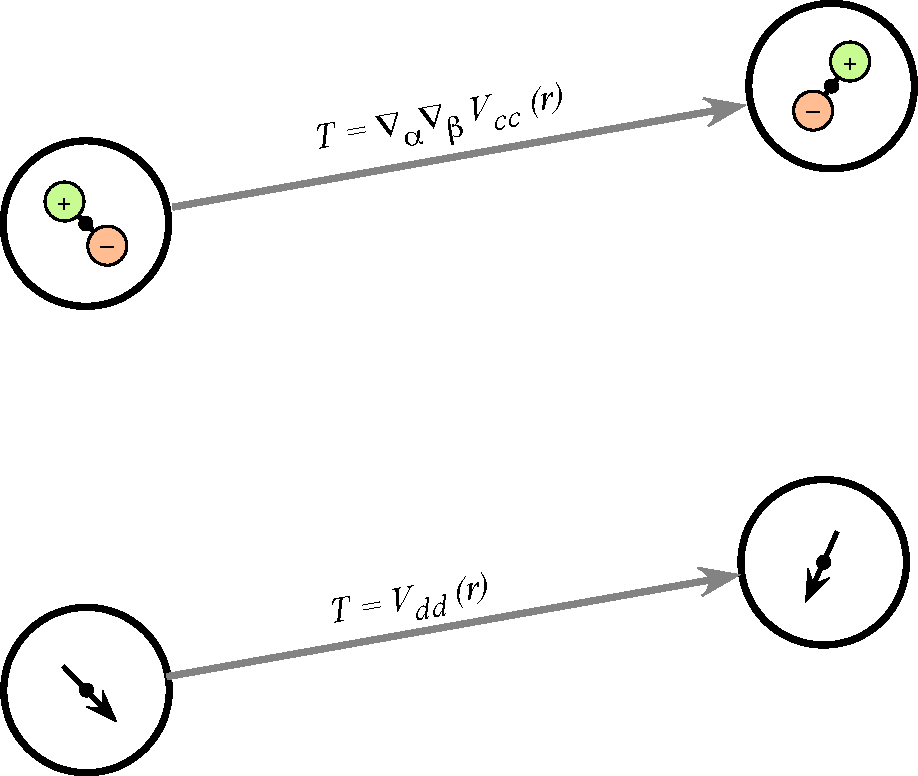
\includegraphics[width=\linewidth]{DielectricFigure}
\caption{With the real-space electrostatic methods, the effective
  dipole tensor, $\mathbf{T}$, governing interactions between
  molecular dipoles is not the same for charge-charge interactions as
  for point dipoles.}
\label{fig:stockmayer}
\end{figure}
In the case where point charges are interacting via an electrostatic
kernel, $v(r)$, the effective {\it molecular} dipole tensor,
$\mathbf{T}$ is obtained from two successive applications of the
gradient operator to the electrostatic kernel,
\begin{equation}
\mathbf{T}_{\alpha \beta}(r) =  \nabla_\alpha \nabla_\beta \left(v(r)\right) = \delta_{\alpha \beta}
\left(\frac{1}{r} v^\prime(r) \right) + \frac{r_{\alpha}
  r_{\beta}}{r^2} \left( v^{\prime \prime}(r) - \frac{1}{r}
  v^{\prime}(r) \right)
\label{dipole-chargeTensor}
\end{equation}
where $v(r)$ may be either the bare kernel ($1/r$) or one of the
modified (Wolf or DSF) kernels.  This tensor describes the effective
interaction between molecular dipoles ($\mathbf{D}$) in Gaussian
units as $-\mathbf{D} \cdot \mathbf{T} \cdot \mathbf{D}$.
When utilizing the new real-space methods for point dipoles, the
tensor is explicitly constructed,
\begin{equation}
\mathbf{T}_{\alpha \beta}(r)  =  \delta_{\alpha \beta} v_{21}(r) +
\frac{r_{\alpha} r_{\beta}}{r^2} v_{22}(r) 
\label{dipole-diopleTensor}
\end{equation}
where the functions $v_{21}(r)$ and $v_{22}(r)$ depend on the level of
the approximation. Although the Taylor-shifted (TSF) and
gradient-shifted (GSF) models produce to the same $v(r)$ function for
point charges, they have distinct forms for the dipole-dipole
interactions.
 
Using constitutive relation, the polarization density $\textbf{P}(\textbf{r})$ is given by,
\begin{equation}
\textbf{P}(\textbf{r}) = \epsilon_o\; \chi^*_D \left(\textbf{E}^o(\textbf{r}) + \frac{1}{4\pi\epsilon_o} \int d^3r' \textbf{T}(\textbf{r}-\textbf{r}')\cdot {\textbf{P}(\textbf{r}')}\right).
\label{constDipole}
\end{equation}
Here $\chi^*_D$ is a dipolar susceptibility can be expressed in terms of dielectric constant as $ \chi^*_D = \epsilon - 1$ which different than macroscopic dipolar polarizability $\alpha_D$ in the sections \ref{subsec:perturbation} and \ref{subsec:fluctuation}. We can split integral into two parts: singular part i.e $|\textbf{r}-\textbf{r}'|\rightarrow 0 $ and non-singular part i.e $|\textbf{r}-\textbf{r}'| > 0 $ . The singular part of the integral can be written as,\cite{NeumannI83, Jackson98}
\begin{equation}
\frac{1}{4\pi\epsilon_o} \int_{|\textbf{r}-\textbf{r}'| \rightarrow 0} d^3r'\; \textbf{T}(\textbf{r}-\textbf{r}')\cdot {\textbf{P}(\textbf{r}')} = - \frac{\textbf{P}(\textbf{r})}{3\epsilon_o}
\label{singular}
\end{equation}
Substituting equation (\ref{singular}) in the equation (\ref{constDipole}) we get,
\begin{equation}
\textbf{P}(\textbf{r}) = 3 \epsilon_o\; \frac{\chi^*_D}{\chi^*_D + 3} \left(\textbf{E}^o(\textbf{r}) + \frac{1}{4\pi\epsilon_o} \int_{|\textbf{r}-\textbf{r}'| > 0} d^3r'\; \textbf{T}(\textbf{r}-\textbf{r}')\cdot {\textbf{P}(\textbf{r}')}\right).
\end{equation}
For both polarization and electric field homogeneous, this can be easily solved using Fourier transformation, 
\begin{equation}
\textbf{P}(\kappa) = 3 \epsilon_o\; \frac{\chi^*_D}{\chi^*_D + 3} \left(1-  \frac{3}{4\pi}\;\frac{\chi^*_D}{\chi^*_D + 3}\; \textbf{T}({\kappa})\right)^{-1}\textbf{E}^o({\kappa}).
\end{equation}
For homogeneous applied field Fourier component is non-zero only if $\kappa = 0$. Therefore,
\begin{equation}
\textbf{P}(0) = 3 \epsilon_o\; \frac{\chi^*_D}{\chi^*_D + 3} \left(1-  \frac{\chi^*_D}{\chi^*_D + 3}\; A_{dipole})\right)^{-1}\textbf{E}^o({0}).
\label{fourierDipole}
\end{equation}
where $A_{dipole}=\frac{3}{4\pi}T(0) = \frac{3}{4\pi} \int_V d^3r\;T(r)$. Now  equation (\ref{fourierDipole}) can be compared with equation (\ref{flucDipole}). Therefore,
\begin{equation}
\frac{\braket{\bf{M}^2}-{\braket{\bf{M}}}^2}{3 \epsilon_o V k_B T} = \frac{3\;\chi^*_D}{\chi^*_D + 3} \left(1-  \frac{\chi^*_D}{\chi^*_D + 3}\; A_{dipole})\right)^{-1}
\end{equation}
Substituting $\chi^*_D = \epsilon-1$ and $ \frac{\braket{\bf{M}^2}-{\braket{\bf{M}}}^2}{3 \epsilon_o V k_B T} = \epsilon_{CB}-1 = \alpha_D$ in above equation we get,
\begin{equation}
\epsilon = \frac{3+(A_{dipole} + 2)(\epsilon_{CB}-1)}{3+(A_{dipole} -1)(\epsilon_{CB}-1)} = \frac{3+(A_{dipole} + 2)\alpha_D}{3+(A_{dipole} -1)\alpha_D}
\label{correctionFormula}
\end{equation}
where $\epsilon_{CB}$ is dielectric constant obtained from conducting boundary condition. Equation (\ref{correctionFormula}) calculates actual dielectric constant from the dielectric constant obtained from the conducting boundary condition (which can be obtained directly from the simulation) using correction factor. The correction factor is different for different real-space cutoff methods. The expression for correction factor assuming a single point dipole or two closely spaced point charges for SP, GSF, and TSF method is listed in Table \ref{tab:A}.

\begin{table}
  \caption{Expressions for the dipolar correction factor ($A$) for the real-space electrostatic methods in terms of the damping parameter
    ($\alpha$) and the cutoff radius ($r_c$).  The Ewald-Kornfeld result 
    derived in Refs. \cite{Adams80,Adams81,NeumannI83} is shown for comparison using the Ewald convergence parameter ($\kappa$) and the real-space cutoff value ($r_c$). }
\label{tab:A}
{
\begin{tabular}{l|c|c|c|}
       
Method & $A_\mathrm{charges}$ & $A_\mathrm{dipoles}$  \\
\hline
Spherical Cutoff (SC) & $\mathrm{erf}(r_c \alpha) - \frac{2 \alpha r_c}{\sqrt{\pi}} e^{-\alpha^2 r_c^2}$ & $\mathrm{erf}(r_c \alpha) - \frac{2 \alpha r_c}{\sqrt{\pi}} e^{-\alpha^2 r_c^2}$ \\
Shifted Potental (SP) & $ \mathrm{erf}(r_c \alpha) - \frac{2 \alpha r_c}{\sqrt{\pi}} e^{-\alpha^2 r_c^2}$ & $\mathrm{erf}(r_c \alpha) -\frac{2 \alpha r_c}{\sqrt{\pi}}\left(1+\frac{2\alpha^2 {r_c}^2}{3} \right)e^{-\alpha^2{r_c}^2} $\\
Gradient-shifted  (GSF) & 1 & $\mathrm{erf}(\alpha  r_c)-\frac{2 \alpha  r_c}{\sqrt{\pi}}  \left(1 + \frac{2 \alpha^2 r_c^2}{3} + \frac{\alpha^4 r_c^4}{3}\right)e^{-\alpha^2 r_c^2} $ \\
Taylor-shifted  (TSF) & 1 & 1 \\ 
Ewald-Kornfeld (EK) & $\mathrm{erf}(r_c \kappa) - \frac{2 \kappa r_c}{\sqrt{\pi}} e^{-\kappa^2 r_c^2}$ & $\mathrm{erf}(r_c \kappa) - \frac{2 \kappa r_c}{\sqrt{\pi}} e^{-\kappa^2 r_c^2}$ \\\hline
\end{tabular}
}
\end{table}    

\subsection{Quadrupolar system}
In the presence of the field gradient $\partial_\alpha {E}_\beta $, a
non-vanishing quadrupolar polarization (quadrupole moment per unit
volume) $\bar{Q}_{\alpha\beta}$ will be induced in the entire volume
of a sample. The total field at any point $\vec{r}$ in the sample is
given by,
\begin{equation}
\partial_\alpha E_\beta(\textbf{r}) = \partial_\alpha {E^o}_\beta(\textbf{r}) + \frac{1}{4\pi \epsilon_o}\int T_{\alpha\beta\gamma\delta}(|{\textbf{r}-\textbf{r}'}|)\;{Q}_{\gamma\delta}(\textbf{r}')\; d^3r'
\label{gradMaxwell}
\end{equation}
where $\partial_\alpha {E^o}_\beta$ is the applied field gradient and $ T_{\alpha\beta\gamma\delta}$ is the quadrupole-quadrupole interaction tensor. We can represent quadrupole as a group of four closely spaced charges, two closely spaced point dipoles or single point quadrupole (see Fig. \ref{fig:quadrupolarFluid}). The quadrupole-quadrupole interaction tensor from the charge representation can obtained from the application of the four successive gradient operator to the electrostatic kernel $v(r)$. 

\begin{equation}
\begin{split}
T_{\alpha\beta\gamma\delta}(r) &=\nabla_\alpha \nabla_\beta \nabla_\gamma \nabla_\delta\;v(r) 
\\ &= \left(\delta_{\alpha\beta}\delta_{\gamma\delta} + \delta_{\alpha\gamma}\delta_{\beta\delta}+ \delta_{\alpha\delta}\delta_{\beta\gamma}\right)\left(-\frac{v'(r)}{r^3} + \frac{v''(r)}{r^2}\right) 
\\ &+ \left(\delta_{\alpha\beta} r_\gamma r_\delta + 5 \; permutations \right) \left(\frac{3v'(r)}{r^5}-\frac{3v''(r)}{r^4} + \frac{v'''(r)}{r^3}\right) 
\\ &+ r_\alpha r_\beta r_\gamma r_\delta\; \left(-\frac{15v'(r)}{r^7}+\frac{15v''(r)}{r^6}-\frac{6v'''(r)}{r^5} + \frac{v''''(r)}{r^4}\right), 
\end{split}
\label{quadCharge}
\end{equation}
where $v(r)$ can either be electrostatic kernel for spherical truncation or one of the modified (Wolf or DSF) method. Similarly in point dipole representation the qaudrupole-quadrupole interaction tensor can be obtained from the applications of the two successive gradient in the dipole-dipole interaction tensor,

\begin{equation}
\begin{split}
T_{\alpha\beta\gamma\delta}(r) &=\nabla_\alpha \nabla_\beta \;v_{\gamma\delta}(r) 
\\ &= \delta_{\alpha\beta}\delta_{\gamma\delta} \frac{v'_{21}(r)}{r} + \left(\delta_{\alpha\gamma}\delta_{\beta\delta}+ \delta_{\alpha\delta}\delta_{\beta\gamma}\right)\frac{v_{22}(r)}{r^2} 
\\ &+ \delta_{\gamma\delta} r_\alpha r_\beta \left(\frac{v''_{21}(r)}{r^2}-\frac{v'_{21}(r)}{r^3} \right)
\\ &+\left(\delta_{\alpha\beta} r_\gamma r_\delta + \delta_{\alpha\gamma} r_\beta r_\delta  +\delta_{\alpha\delta} r_\gamma r_\beta + \delta_{\beta\gamma} r_\alpha r_\delta +\delta_{\beta\delta} r_\alpha r_\gamma  \right) \left(\frac{v'_{22}(r)}{r^3}-\frac{2v_{22}(r)}{r^4}\right) 
\\ &+ r_\alpha r_\beta r_\gamma r_\delta\; \left(\frac{v''_{22}(r)}{r^4}-\frac{5v'_{22}(r)}{r^5}+\frac{8v_{22}(r)}{r^6}\right), 
\end{split}
\label{quadDip}
\end{equation}
where $v_{\gamma\delta}(r)$ is the electrostatic dipole-dipole interaction tensor, which is different for different electrostatic cut off methods. Similarly $v_{21}(r) \;and\; v_{22}(r)$ are the radial function for different real space cutoff methods defined in Paper I of the series.\cite{PaperI} Using point quadrupole representation the quadrupole-quadrupole interaction can be constructed as,  
\begin{equation}
\begin{split}
T_{\alpha\beta\gamma\delta}(r) &= \left(\delta_{\alpha\beta}\delta_{\gamma\delta} + \delta_{\alpha\gamma}\delta_{\beta\delta}+ \delta_{\alpha\delta}\delta_{\beta\gamma}\right)v_{41}(r) + \delta_{\gamma\delta} r_\alpha r_\beta \frac{v_{42}(r)}{r^2} \\ &+ r_\alpha r_\beta r_\gamma r_\delta\; \left(\frac{v_{43}(r)}{r^4}\right), 
\end{split}
\label{quadRadial}
\end{equation}
where $v_{41}(r),\; v_{42}(r), \; \text{and} \; v_{43}(r)$ are defined in Paper I  of the series. \cite{PaperI} They have  different functional forms for different electrostatic cutoff methods.
\begin{figure}
  \centering
  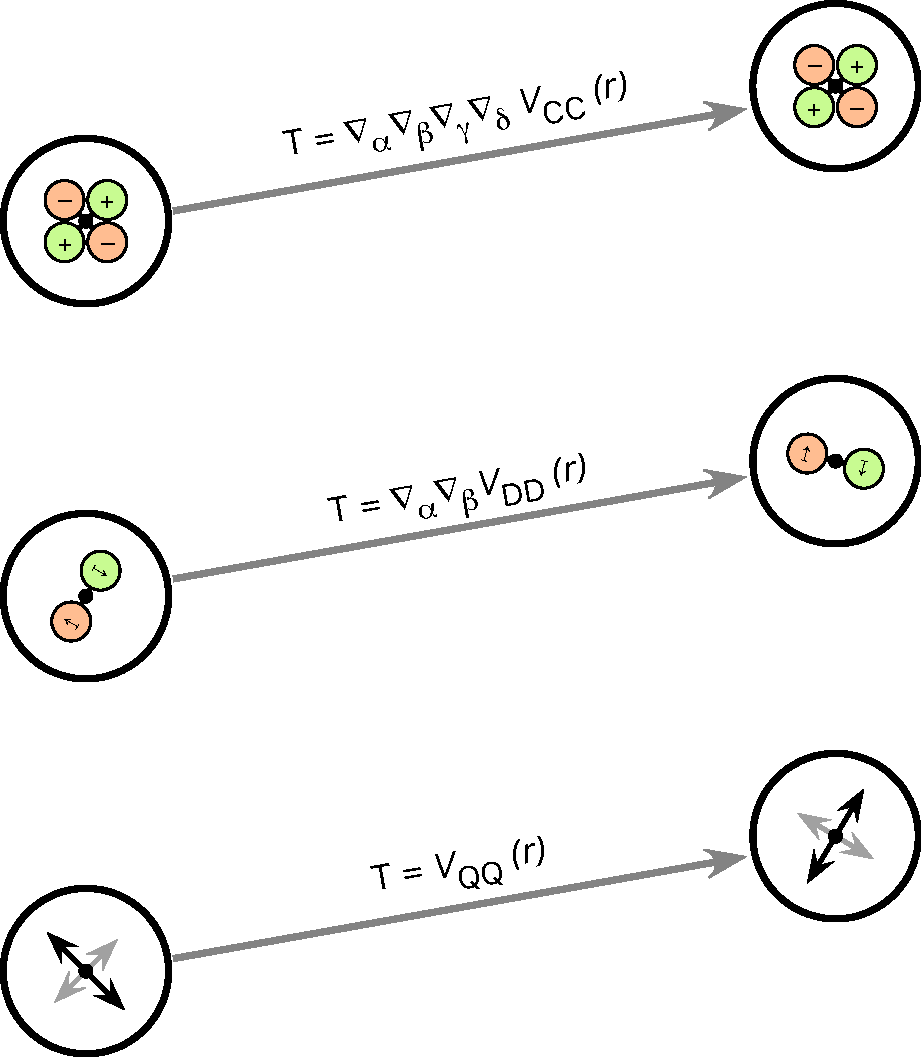
\includegraphics[width=\linewidth]{QuadrupoleFigure}
\caption{With the real-space electrostatic methods, the effective
  quadrupolar tensor, $\mathbf{T}_{\alpha\beta\gamma\delta}(r)$, governing interactions between molecular quadrupoles can be represented by interaction of charges, point dipoles or single point quadrupoles.}
\label{fig:quadrupolarFluid}
\end{figure}

The integral in equation (\ref{gradMaxwell}) can be divided into two parts, $|\textbf{r}-\textbf{r}'|\rightarrow 0 $ and $|\textbf{r}-\textbf{r}'|> 0$. Since the total
field gradient due to quadrupolar fluid vanishes at the singularity (see Appendix \ref{singularQuad}), equation (\ref{gradMaxwell}) can be written as,
\begin{equation}
\partial_\alpha E_\beta(\textbf{r}) = \partial_\alpha {E^o}_\beta(\textbf{r}) +
  \frac{1}{4\pi \epsilon_o}\int\limits_{|\textbf{r}-\textbf{r}'|> 0 }
  T_{\alpha\beta\gamma\delta}(|\textbf{r}-\textbf{r}'|)\;{Q}_{\gamma\delta}(\textbf{r}')\;
  d^3r'. 
\end{equation}
If $\textbf{r} = \textbf{r}'$ is excluded from the integration, the gradient of the electric can be expressed in terms of traceless quadrupole moment as below, \cite{LoganI81}
\begin{equation}
\partial_\alpha E_\beta(\textbf{r}) = \partial_\alpha {E^o}_\beta(\textbf{r}) + \frac{1}{12\pi \epsilon_o}\int\limits_{|\textbf{r}-\textbf{r}'|> 0 } T_{\alpha\beta\gamma\delta}(|\textbf{r}-\textbf{r}'|)\;{\Theta}_{\gamma\delta}(\textbf{r}')\; d^3r',
\end{equation}
where $\Theta_{\alpha\beta} = 3Q_{\alpha\beta} - \delta_{\alpha\beta}Tr(Q)$
is the traceless quadrupole moment. The total quadrupolar polarization is written as,
\begin{equation}
{Q}_{\alpha\beta}(\textbf{r}) =  \frac{1}{3}\delta_{\alpha\beta}\;Tr({Q})+\epsilon_o {\chi}^*_Q\;\partial_\alpha E_\beta(\textbf{r}),
\label{constQaud}
\end{equation}
In the equation (\ref{constQaud}), $\partial_{\alpha}E_{\beta}$ is Maxwell field gradient and ${\chi}^*_Q$ is the actual quadrupolar susceptibility of the fluid which is different than the proportionality constant $\chi_q $ in the equation (\ref{propConstQuad}). In terms of traceless quadrupole moment, equation (\ref{constQaud}) can be written as,
\begin{equation}
\frac{1}{3}{\Theta}_{\alpha\beta}(\textbf{r}) =  \epsilon_o {\chi}^*_Q \; \partial_\alpha E_\beta (\textbf{r})=  \epsilon_o {\chi}^*_Q \left(\partial_\alpha {E^o}_\beta(\textbf{r}) + \frac{1}{12\pi \epsilon_o}\int\limits_{|\textbf{r}-\textbf{r}'|> 0 } T_{\alpha\beta\gamma\delta}(|\textbf{r}-\textbf{r}'|)\;{\Theta}_{\gamma\delta}(\textbf{r}')\; d^3r'\right)
\end{equation}
For toroidal boundary conditions, both $\partial_\alpha E_\beta$ and
${\Theta}_{\alpha\beta}$ are uniform over the entire space. After
performing a Fourier transform (see the Appendix in the Neumann's Paper  \cite{NeumannI83}) we get,
\begin{equation}
\frac{1}{3}{{\Theta}}_{\alpha\beta}({\kappa})=
\epsilon_o {\chi}^*_Q \;\left[{\partial_\alpha
    {E^o}_\beta}({\kappa})+ \frac{1}{12\pi
    \epsilon_o}\;{T}_{\alpha\beta\gamma\delta}({\kappa})\;
 {{\Theta}}_{\gamma\delta}({\kappa})\right] 
\end{equation} 
Since the quadrupolar polarization is in the direction of the applied
field, we can write
${{\Theta}}_{\gamma\delta}({\kappa}) =
{{\Theta}}_{\alpha\beta}({\kappa})$
and
${T}_{\alpha\beta\gamma\delta}({\kappa}) =
{T}_{\alpha\beta\alpha\beta}({\kappa})$. Therefore we can consider each component of the interaction tensor as scalar and perform calculation.
\begin{equation}
\begin{split}
\frac{1}{3}{{\Theta}}_{\alpha\beta}({\kappa}) &= \epsilon_o {\chi}^*_Q \left[{\partial_\alpha E^o_\beta}({\kappa})+ \frac{1}{12\pi \epsilon_o}{T}_{\alpha\beta\alpha\beta}({\kappa})\;{{\Theta}}_{\alpha\beta}({\kappa})\right] \\
&= \epsilon_o {\chi}^*_Q\;\left(1-\frac{1}{4\pi} {\chi}^*_Q\;
 {T}_{\alpha\beta\alpha\beta}({\kappa})\right)^{-1}
{\partial_\alpha E^o_\beta}({\kappa}) 
\end{split}
\label{fourierQuad}
\end{equation} 
If the field gradient is homogeneous over the
entire volume, ${\partial_ \alpha E_\beta}({\kappa}) = 0 $ except at
$ {\kappa} = 0$, hence it is sufficient to know
${T}_{\alpha\beta\alpha\beta}({\kappa})$ at $ {\kappa} =
0$. Therefore equation (\ref{fourierQuad}) can be written as,
\begin{equation}
\begin{split}
\frac{1}{3}{{\Theta}}_{\alpha\beta}({0}) &= \epsilon_o {\chi}^*_Q\; \left(1-\frac{1}{4\pi} {\chi}^*_Q\;{T}_{\alpha\beta\alpha\beta}({0})\right)^{-1} \partial_\alpha E^o_\beta({0})
\end{split}
\label{fourierQuad2}
\end{equation}
where $ {T}_{\alpha\beta\alpha\beta}({0})$ can be evaluated as,
\begin{equation}
{T}_{\alpha\beta\alpha\beta}({0}) = \int {T}_{\alpha\beta\alpha\beta}\;(\textbf{r})d^3r
\label{realTensorQaud}
\end{equation}

In terms of traced quadrupole moment equation (\ref{fourierQuad2}) can be written as,
\begin{equation}
{{Q}}_{\alpha\beta} = \frac{1}{3}\delta_{\alpha\beta}\;Tr({Q}) + \epsilon_o\; {\chi}^*_Q\left(1-\frac{1}{4\pi} {\chi}^*_Q\;{T}_{\alpha\beta\alpha\beta}({0})\right)^{-1}\; \partial_\alpha E^o_\beta
\label{tracedConstQuad}
\end{equation}
Comparing (\ref{tracedConstQuad}) and (\ref{flucQuad}) we get,
\begin{equation}
\begin{split}
&\frac{\braket{{Q^2}} - \braket{Q}^2}{15 \epsilon_o Vk_BT}\; =\; {\chi}^*_Q\;\left(1-\frac{1}{4\pi} {\chi}^*_Q\;{T}_{\alpha\beta\alpha\beta}({0})\right)^{-1}, \\ 
&{\chi}^*_Q \;=\; \frac{\braket{{Q^2}} - \braket{Q}^2}{15 \epsilon_o Vk_BT}\left(1 + \frac{1}{4\pi} \frac{\braket{{Q^2}} - \braket{Q}^2}{15 \epsilon_o Vk_BT}\;{T}_{\alpha\beta\alpha\beta}({0})\right)^{-1}
\end{split}
\end{equation}
Finally the quadrupolar susceptibility cab be written in terms of quadrupolar correction factor ($A_{quad}$) as below, 
\begin{equation}
{\chi}^*_Q \;=\; \frac{\braket{{Q^2}} - \braket{Q}^2}{15 \epsilon_o Vk_BT}\left(1 + \frac{\braket{{Q^2}} - \braket{Q}^2}{15 \epsilon_o Vk_BT}\; A_{quad}\right)^{-1} = \alpha_Q\left(1 + \alpha_Q\; A_{quad}\right)^{-1}
\label{eq:quadrupolarSusceptiblity}
\end{equation}
where $A_{quad} = \frac{1}{4\pi}\int {T}_{\alpha\beta\alpha\beta}\;(\textbf{r})d^3r $ has dimension of the $length^{-2}$ is different for different cutoff methods which is listed in Table \ref{tab:B}. The dielectric constant associated with the quadrupolar susceptibility is defined as,\cite{Ernst92}

\begin{equation}
\epsilon = 1 + \chi^*_Q\; G = 1 + G \; \alpha_Q\left(1 + \alpha_Q\;  A_{quad}\right)^{-1}
\label{eq:dielectricFromQuadrupoles}
\end{equation}
where $G = \frac{\displaystyle\int_V |\partial_\alpha E^o_\beta|^2 d^3r}{\displaystyle\int_V{|E^o|}^2 d^3r}$ is a geometrical factor depends on the nature of the external field perturbation. This is true when the quadrupolar fluid is homogeneous over the sample. Since quadrupolar molecule couple with the gradient of the field, the distribution of the quadrupoles is inhomogeneous for varying field gradient. Hence the distribution function should also be taken into account to calculate actual geometrical factor in the presence of non-uniform gradient field. Therefore,
\begin{equation}
G = \frac{\displaystyle\int_V\; g(r, \theta, \phi)\; |\partial_\alpha E^o_\beta|^2 d^3r}{\displaystyle\int_V{|E^o|}^2 d^3r}
\label{eq:geometricalFactor}
\end{equation}
where $g(r,\theta, \phi)$ is a distribution function of the quadrupoles in with respect to origin at the center of line joining two probe charges.  

\begin{sidewaystable}
  \caption{Expressions for the quadrupolar correction factor ($A$) for the real-space electrostatic methods in terms of the damping parameter
    ($\alpha$) and the cutoff radius ($r_c$). The dimension of the correction factor is $ length^{-2}$ in case of quadrupolar fluid.}
\label{tab:B}
\centering
\resizebox{\columnwidth}{!}{

\begin{tabular}{l|c|c|c|c|} \hline
       
Method & $A_\mathrm{charges}$ & $A_\mathrm{dipoles}$ &$A_\mathrm{quadrupoles}$  \\\hline
Spherical Cutoff (SC) & $ -\frac{8 \alpha^5 {r_c}^3}{3\sqrt{\pi}} e^{-\alpha^2 r_c^2}$ &  $ -\frac{8 \alpha^5 {r_c}^3}{3\sqrt{\pi}} e^{-\alpha^2 r_c^2}$ & $ -\frac{8 {\alpha}^5 {r_c}^3}{3\sqrt{\pi}} e^{-\alpha^2 r_c^2}$ \\
Shifted Potental (SP) & $ -\frac{8 \alpha^5 {r_c}^3}{3\sqrt{\pi}} e^{-\alpha^2 r_c^2}$ &  $- \frac{8 \alpha^5 {r_c}^3}{3\sqrt{\pi}} e^{-\alpha^2 r_c^2}$& $ -\frac{16 \alpha^7 {r_c}^5}{9\sqrt{\pi}} e^{-\alpha^2 r_c^2}$  \\
Gradient-shifted  (GSF) & $- \frac{8 \alpha^5 {r_c}^3}{3\sqrt{\pi}} e^{-\alpha^2 r_c^2}$ & 0 &  $-\frac{4{\alpha}^7{r_c}^5 }{9\sqrt{\pi}}e^{-\alpha^2 r_c^2}(-1+2\alpha ^2 r_c^2)$\\
Taylor-shifted  (TSF) &  $ -\frac{8 \alpha^5 {r_c}^3}{3\sqrt{\pi}} e^{-\alpha^2 r_c^2}$ & $\frac{4\;\mathrm{erfc(\alpha r_c)}}{{r_c}^2} + \frac{8 \alpha}{3\sqrt{\pi}r_c}e^{-\alpha^2 {r_c}^2}\left(3+ 2 \alpha^2 {r_c}^2 + \alpha^4 {r_c}^4\right)  $ & $\frac{10\;\mathrm{erfc}(\alpha r_c )}{{r_c}^2} + \frac{4{\alpha}}{9\sqrt{\pi}{r_c}}e^{-\alpha^2 r_c^2}\left(45 + 30\alpha ^2 {r_c}^2 + 12\alpha^4 {r_c}^4 + 3\alpha^6 {r_c}^6 + 2 \alpha^8 {r_c}^8\right)$ \\\hline
\end{tabular}
}
\end{sidewaystable}

\section{Methodology}
We have used three different simulation methods: i) external field perturbation, ii) fluctuation formula, and iii) potential of mean force (PMF), to calculate dielectric properties for dipolar and quadrupolar fluid. For the dipolar system we calculated macroscopic polarzability using first two methods and derived the dielectric constant using polarizability and correction factor (see equation \ref{correctionFormula}). Similarly we used equation (\ref{eq:pmf}) to calculate screening factor from dipolar fluid using PMF method. For quadrupolar fluid, we have calculated quadrupolarizablity using fluctuation formula and external field perturbation and derived quadrupolar susceptibility using quadrupolarizability and correction factor (equation \ref{eq:quadrupolarSusceptiblity}). Since dielectric constant due to quadrupolar fluid depends on the nature of gradient of the field applied in the system, we have used geometrical factor (in equation \ref{eq:geometricalFactor}) and quadrupolar susceptibility to evaluate dielectric constant for two ions dissolved quadrupolar fluid (see equation \ref{eq:dielectricFromQuadrupoles}) . The the dielectric constant evaluated using equation (\ref{eq:dielectricFromQuadrupoles}) has been compared with the result evaluated from PMF method (i.e. equation \ref{eq:pmf}). We have also used three different test systems for both dipolar and quadrupolar fluids to calculate dielectric properties. The parameters used in the test systems are given in table \ref{Tab:C}.
\begin{sidewaystable}
  \caption{The mass, moment of intertia, Lennard-Jones, and electrostatic parameters for the test systems are listed below. \label{Tab:C}}
\begin{tabularx}{\textwidth}{r|cc|YYccc|Yccc} \hline
             & \multicolumn{2}{c|}{LJ parameters} &
             \multicolumn{5}{c|}{Electrostatic moments} & & & & \\
 Test system & $\sigma$& $\epsilon$ & $C$ & $D$  &
 $Q_{xx}$ & $Q_{yy}$ & $Q_{zz}$ & mass  & $I_{xx}$ & $I_{yy}$ &
 $I_{zz}$ \\ \cline{6-8}\cline{10-12}
 & (\AA) & (kcal/mol) & (e) & (debye) & \multicolumn{3}{c|}{(debye \AA)} & (amu) & \multicolumn{3}{c}{(amu
 \AA\textsuperscript{2})} \\ \hline
    Stockmayer fluid & 3.41 & 0.2381 & - & 1.4026 &-&-&-& 39.948 & 11.613 & 11.613 & 0.0 \\
	Quadrupolar fluid & 2.985 & 0.265 & - & - & 0.0 & 0.0 &-2.139 & 18.0153 & 43.0565 & 43.0565 & 0.0  \\
              \ce{q+} & 1.0 & 0.1 & +1 & - & - & - & - & 22.98 & - & - & - \\
              \ce{q-} & 1.0 & 0.1 & -1 & - & - & - & - & 22.98 & - & - & - \\ \hline
\end{tabularx}
\end{sidewaystable}

First test system consists of point dipolar or quadrupolar molecules in the presence of constant field or gradient field. Since there is no isolated charge within the system, the divergence of the field should be zero $ i.e. \vec{\nabla} .\vec{E} = 0$. This condition is satisfied by selecting applied potential as described in Appendix \ref{Ap:fieldOrGradient}.  When constant electric field or field gradient applied to the system, the molecules align along the direction of the applied field. We have calculated ensemble average of the box dipole or quadrupole moment as a response field or field gradient. Similarly the  macroscopic polarizability of the system is derived using ratio between system multipolar moment and applied field or field gradient. This method works properly when the system is at the linear response region of field or field gradient.    

Second test system consists of box of point dipolar or quadrupolar molecules is simulated for 1 ns in NVE ensemble after equilibration in the absence of any external perturbation. The fluctuation of the ensemble average of the box multipolar moment, $\braket{A^2} - \braket{A}^2 $ where A is box dipolar or quadrupolar moment,  is measured at the fixed temperature and density for a given multipolar fluid. Finally the macroscopic polarizability of the system at a particular density is derived using equation (\ref{flucQuad}).

Final system consists of dipolar or quadrupolar fluids with two oppositely charged ions immersed in it. These ions are constraint to be at fixed distance throughout the simulation. We run separate simulations for the different constraint distances. We calculated the screening factor using ratio between the force between the two ions in the absence of medium and the average constraint force during the simulation. Since the constraint force is pretty noisy we run each simulation for long time ($\sim 5$ ns) to reduce simulation error.

\subsection{Implementation}
We have used real-space electrostatic methods implemented in OpenMD \cite{openmd2.3} software to evaluate electrostatic interactions between the molecules. In our simulations we used all three different real-space electrostatic methods: SP, GSF, and TSF developed in the previous paper \cite{PaperI} in the series. The radius of the cutoff sphere is taken to be $12 \r{A}$. Each real space method can be tuned using different values of damping parameter. We have selected ten different values of damping parameter (unit-${\r{A}}^{-1}$); 0.0, 0.05, 0.1, 0.15, 0.175, 0.2, 0.225, 0.25, 0.3, and 0.35 in our simulations for dipolar system. Since quadrupolar interactions are less sensitive to damping parameter as compared to dipole we selected only four values of dampig alpha 0.0, 0.1 0.2, and 0.3 $\AA-1$ in our simulation. The short range interaction in the simulations is incorporated using 6-12 Lennard Jones interactions. 

To derive the box multipolar (dipolar or quadrupolar) moment, we added the component each individual molecule and taken ensemble average of each snapshot in the entire simulation. The first component of the fluctuation of the dipolar moment is derived by using relation $\braket{M^2} = \braket{{M_x}^2 + {M_y}^2 + {M_z}^2}$, where $M_x$, $M_y$, and $M_z $ are x, y and z components of the box dipolar moment. Similarly the first term in the quadrupolar system is derived using relation $ \braket{Q^2} = \braket{3 Q:Q - \mathrm{Tr}Q^2} $, where $ Q $ is the box quadrupole moment, double dot represent the outer product of the quadrupolar matrices, and $TrQ$ is the trace of the box quadrupolar moment. The second component of the fluctuation formula has been derived using square of the ensemble average of the box dipole moment. The applied constant field or field gradient in the test systems has been taken in the form described in the Appendix \ref{Ap:fieldOrGradient}.

\subsection{Model systems}
To evaluate dielectric properties for dipolar systems using perturbation and fluctuation formula methods, we have taken system of 2048 Stockmayer molecules with reduced density $ \rho^* = 0.822$, temperature $T^* = 1.15 $, moment of inertia $I^* =  0.025 $, and dipole moment $ \mu^* = \sqrt{3.0} $. Test systems are equilibrated for 500 ps and run for $1\; ns$ and components of box dipole moment are obtained at every femtosecond. The systems have been run in the presence of constant external field from $ 0 - 10\; \times\; 10^{-4}\;V/{\r{A}}$ in the step of $ 10 ^{-4}\; V/\r{A}$ for each simulation. For pmf method, Two dipolar molecules in the above system are converted into $q+$ and $q-$ ions and constrained to remain in fixed distance in simulation. The constrained distance is varied from $5\;\r{A} - 12\; \r{A} $ for different simulations. In pmf method all simulations are equilibrated for 500 ps in NVT ensemble and run for 5 ns in NVE ensemble to print constraint force at an interval of 20 fs.   

Quadrupolar systems consists 4000 linear point quadrupoles with density $ 2.338\; g/cm^3$ at temperature $ 500\; ^oK $. For both perturbation and fluctuation methods, test systems are equalibrated for 200 ps in NVT ensemble and run for 500 ps in NVE ensemble. To find the ensemble average of the box quadrupole moment and fluctuation, the components of box quadrupole moments are printed every 100 fs. Each simulations repeated at different values of applied gradients from $ 0 - 9 \times 10^{-2}\; V/\AA^2 $. To calculate dielectric constant using pmf method, two ions in the systems are converted into $q+$ and $q-$ ions and constrained to remain at fixed distance in the simulation. These constraint distances are varied from $5\;\AA - 12\; \AA $ at the step of $0.1\; \AA $ for different simulations. For calculating dielectric constant, the test systems are run for 500 ps to equlibrate and run for 5 ns to print constraint force at a time interval of 20 fs.

\section{Results}
\subsection{Dipolar fluid}
The macroscopic polarizability ($\alpha_D$) for Stockmayer fluid evaluated using perturbation (left) and fluctuation (right) methods as shown in figure \ref{fig:dielectricDipole} . The polarizability obtained from the both perturbation and fluctuation methods show excellent agreement with each other. The result shows that polarizability hugely depends on the values of the damping parameter in the case of Shifted Potential (SP) and Gradient Shifted force (GSF) methods. But the results obtained using Taylor Shifted Force (TSF) show slight dependence on the damping alpha.  To get correct dielectric properties from the polarizability we used a correction factor as we discussed in section \ref{sec:corrFactor}. The correction factor for dipolar fluids ($\mathrm{A}_\mathrm{dipole}$ ) for the different values of damping parameter is also plotted in figure \ref{fig:dielectricDipole}. For TSF method, $ \mathrm{A}_\mathrm{dipole} = 1 $ for all the values of damping alpha. Therefore we do not need to perform any correction to obtain dielectric constant from the polarizability. The values of $\mathrm{A}_\mathrm{dipole} $ varies with the damping parameter in the case of SP and GSF methods therefore correction factor should be incorporated to calculate the dielectric constant ($\epsilon$) from the polarzability. The dielectric constant obtained from the polarizability and correction factor is also plotted in the figure \ref{fig:dielectricDipole}. The dielectric constant evaluated using SP and GSF method shows good agreement with the previous simulation result (straight dotted line in the lower panels)\cite{NeumannI83} for the damping parameter from $0.25\; \mathrm{to}\; 0.3$ $\AA-1$. For lower value of the damping alpha the dielectric constant is much deviated away from the previous simulation result. To investigate furthermore we performed inverse transformation of expected dielectric constant \cite{NeumannI83}, using correction factor and calculated expected polarizability for the simulation, which is represented by the dotted line in the upper-left and upper-right panels. In the plot we can clearly see that expected ploarizability for the SP and GSF methods are very close to results obtained from the simulations. Sometime even they are within the range of the error-bar but when the dielectric constant is calculated using simulation result and correction formula, it is found to be deviated much away from the expected result for the lower values of the damping alpha. This tell us that the correction formula (equation \ref{correctionFormula}) for the dipolar fluid is very sensitive when the value of $\mathrm{A}_\mathrm{dipole}$ is deviated much away from 1 for the small values of damping parameter. Therefore it is always better to select damping alpha from 0.25 to 0.3 $\AA^{-1}$ to evaluate dielectric constant using perturbation and fluctuation formula while using SP and GSF methods in simulation.    

\begin{figure}
  \centering
  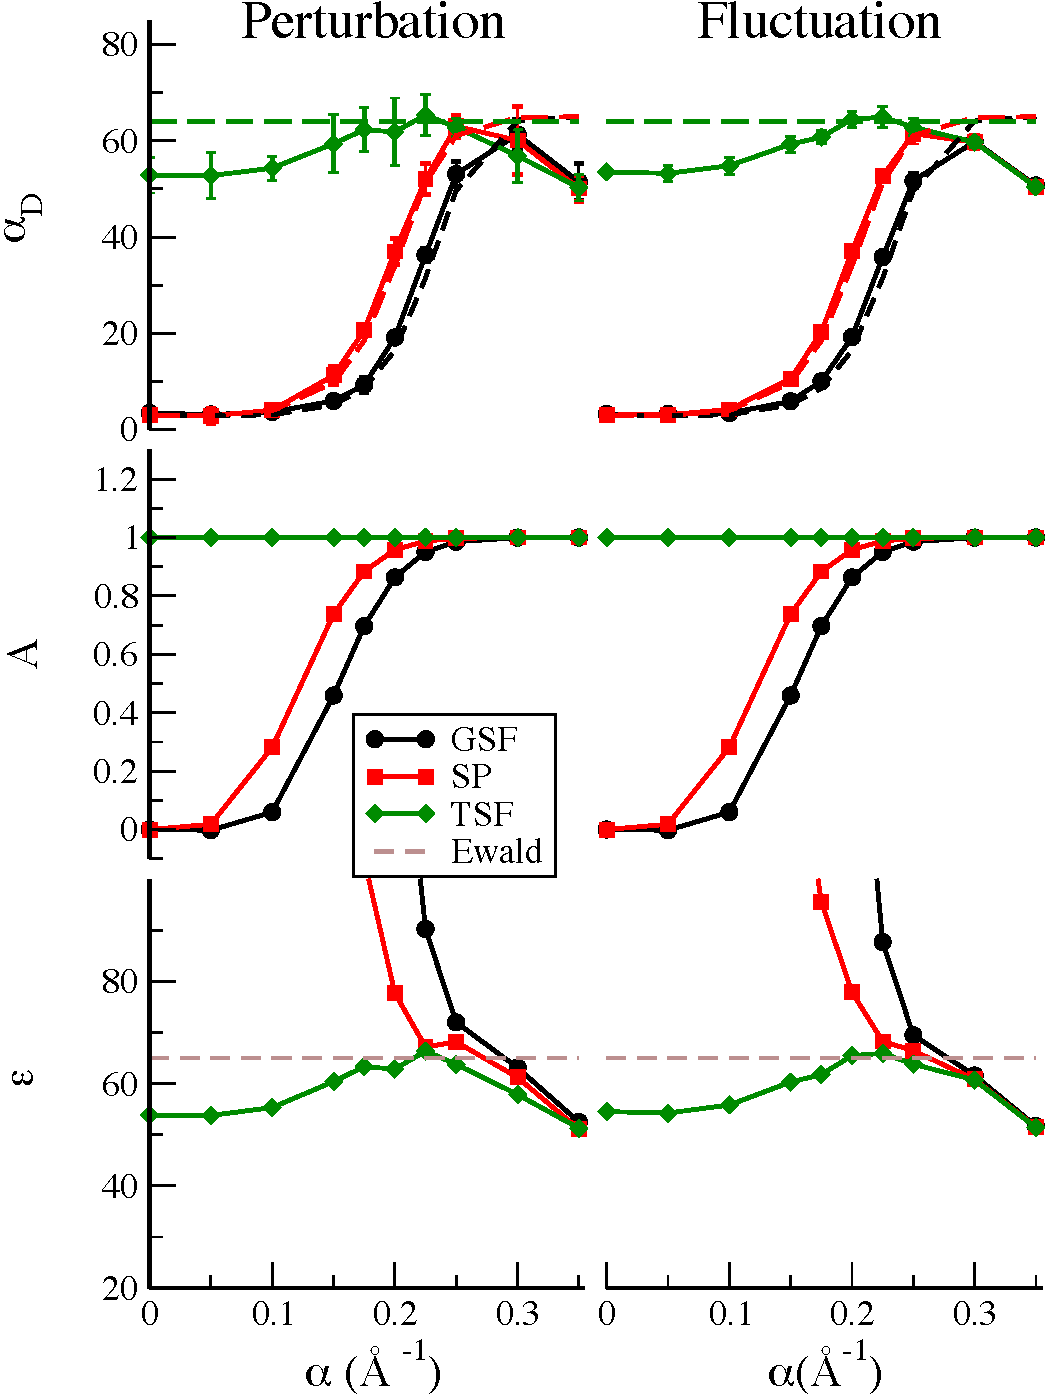
\includegraphics[width=\linewidth]{dielectricFinal_Dipole.pdf}
\caption{In the figure, $\alpha_D$, $\mathrm{A}_\mathrm{dipole}$, and $\epsilon$  are polarizability, correction factor, and dielectric constant for Stockmayer fluid. Plots in the left panel show results for (a) perturbation method and right (b) fluctuation method.}
\label{fig:dielectricDipole}
\end{figure}

We have also evaluated the screening factor between two oppositely charged ions when they are placed in the Stockmayer fluid as shown in figure \ref{fig:ScreeningFactor_Dipole}. The screening factor have been evaluated using equation \ref{eq:pmf}. This screening factor is analogous to dielectric screening but there is subtle differences between them. Actually screening factor measures a local property of the ions in the fluid and depends on ion-dipole and dipole-dipole interactions. These interactions depends on the distance between ions and electrostatic interaction methods implemented in the simulations. But we can expect screening to be close to dielectric constant when the field due to ions is very gentle in perturbation. It is possible when distance between ions are far apart and values of damping parameter relatively higher. In the figure \ref{fig:ScreeningFactor_Dipole} we can observe that for the higher value of damping alpha i.e $\alpha = 0.2 \AA^{-1}$ and $0.3 \AA^{-1}$ and large separation between ions, the screening factor approaches to the dielectric constant. We can also  observe that for TSF method has got higher screening factor as compared SP and GSF method even for lower damping alpha. It is because of dipole-dipole interactions do not need any correction factor in the case of TSF as we discussed earlier. But presence of ion-dipole interaction causing local effect even in the case of TSF method for small ions separation.

\begin{figure}
  \centering
  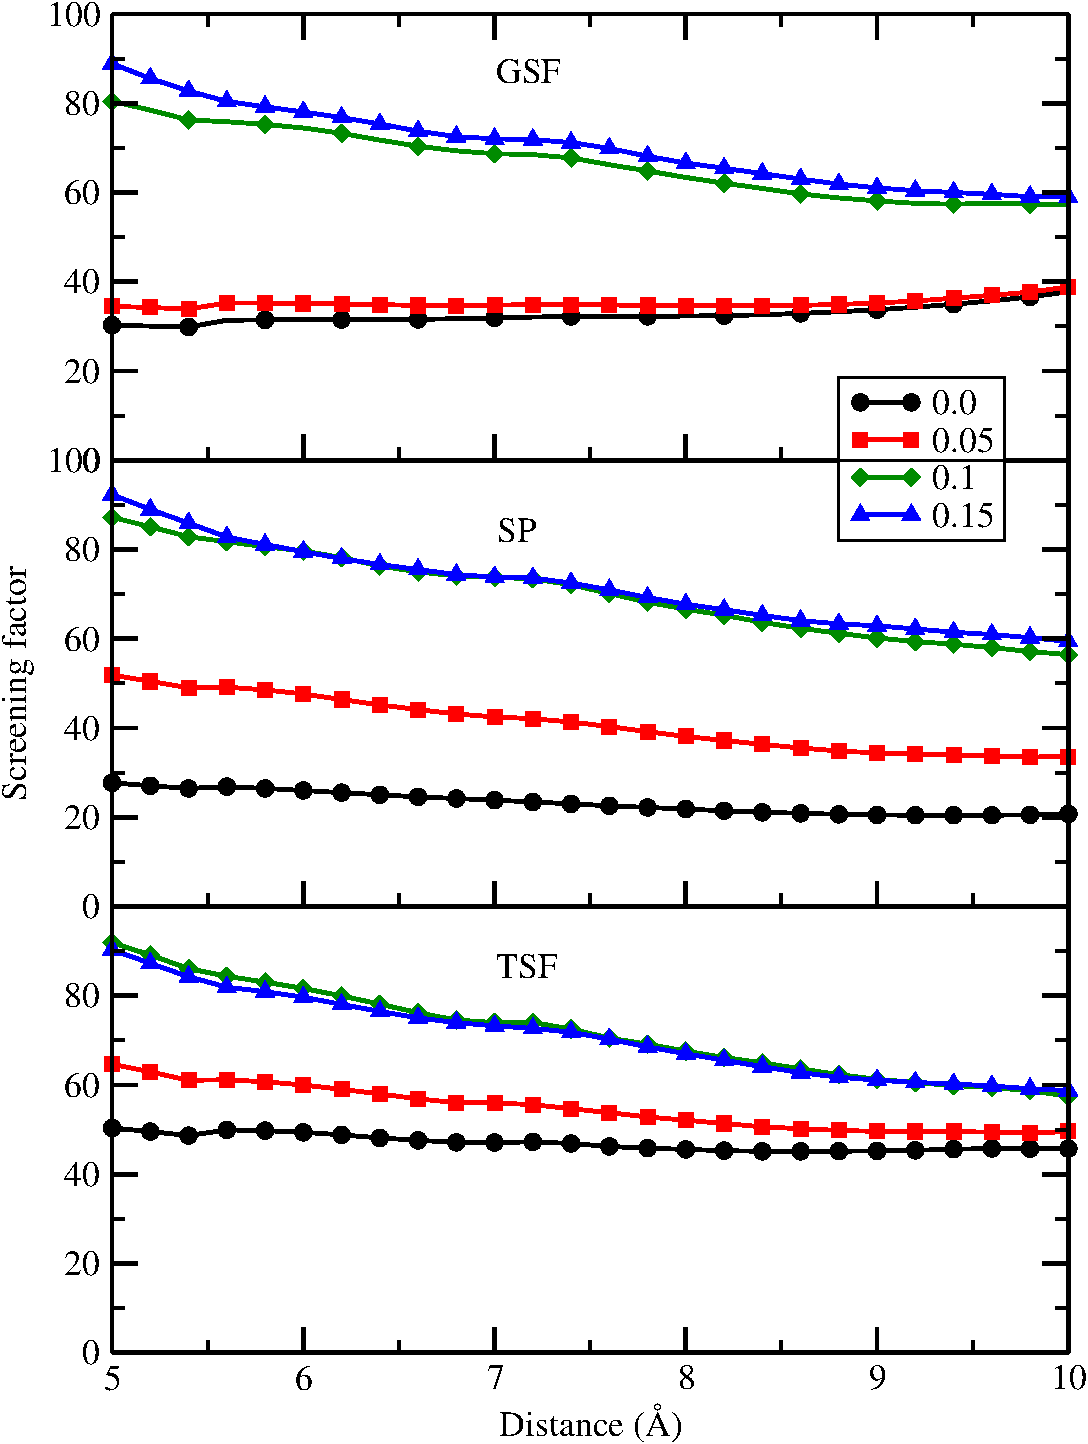
\includegraphics[width=\linewidth]{ScreeningFactor_Dipole.pdf}
\caption{Figure shows screening factor between two oppositely charged ions immersed in Stockmayer fluid as a function of ions-separation for the different values damping alpha and electrostatic methods.}
\label{fig:ScreeningFactor_Dipole}
\end{figure}

\subsection{Quadrupolar fluid}
The polarizability ($\alpha_Q$), correction factor ($\mathrm{A_{quad}}$), and susceptibility ($\chi$) for the quadrupolar fluid is plotted against damping parameter in the figure \ref{fig:dielectricQuad}. Different than the dipolar fluid, the polarizability and susceptibility for the quadrupolar fluid have a dimension of $\AA ^2$. Although susceptibility has got dimension, it is a measure of macroscopic quadrupolar properties at a given temperature and density \cite{JeonI03, JeonII03}. The left panel in the plot showing results obtained from  the perturbation whereas the results from the fluctuation formula are plotted in the right panel. In the figure, we can observe that the polarizablity evaluated from the perturbation (top-left) shows excellent agreement with the result obtained from the fluctuation formula (top-right). The susceptibility for the quadrupolar fluid is obtained from quadrupolarizability and correction factor using equation \ref{eq:quadrupolarSusceptiblity} which is plotted at the bottom-left and bottom-right in the figure \ref{fig:dielectricQuad}. All three methods: SP, GSF, and TSF tends to produce same value of susceptibility for the given value damping alpha. This shows that susceptibility derived using correction factor and polarizablity is tends to be independent of the electrostatic method implemented in the simulation for quadrupolar fluid.

\begin{figure}
  \centering
  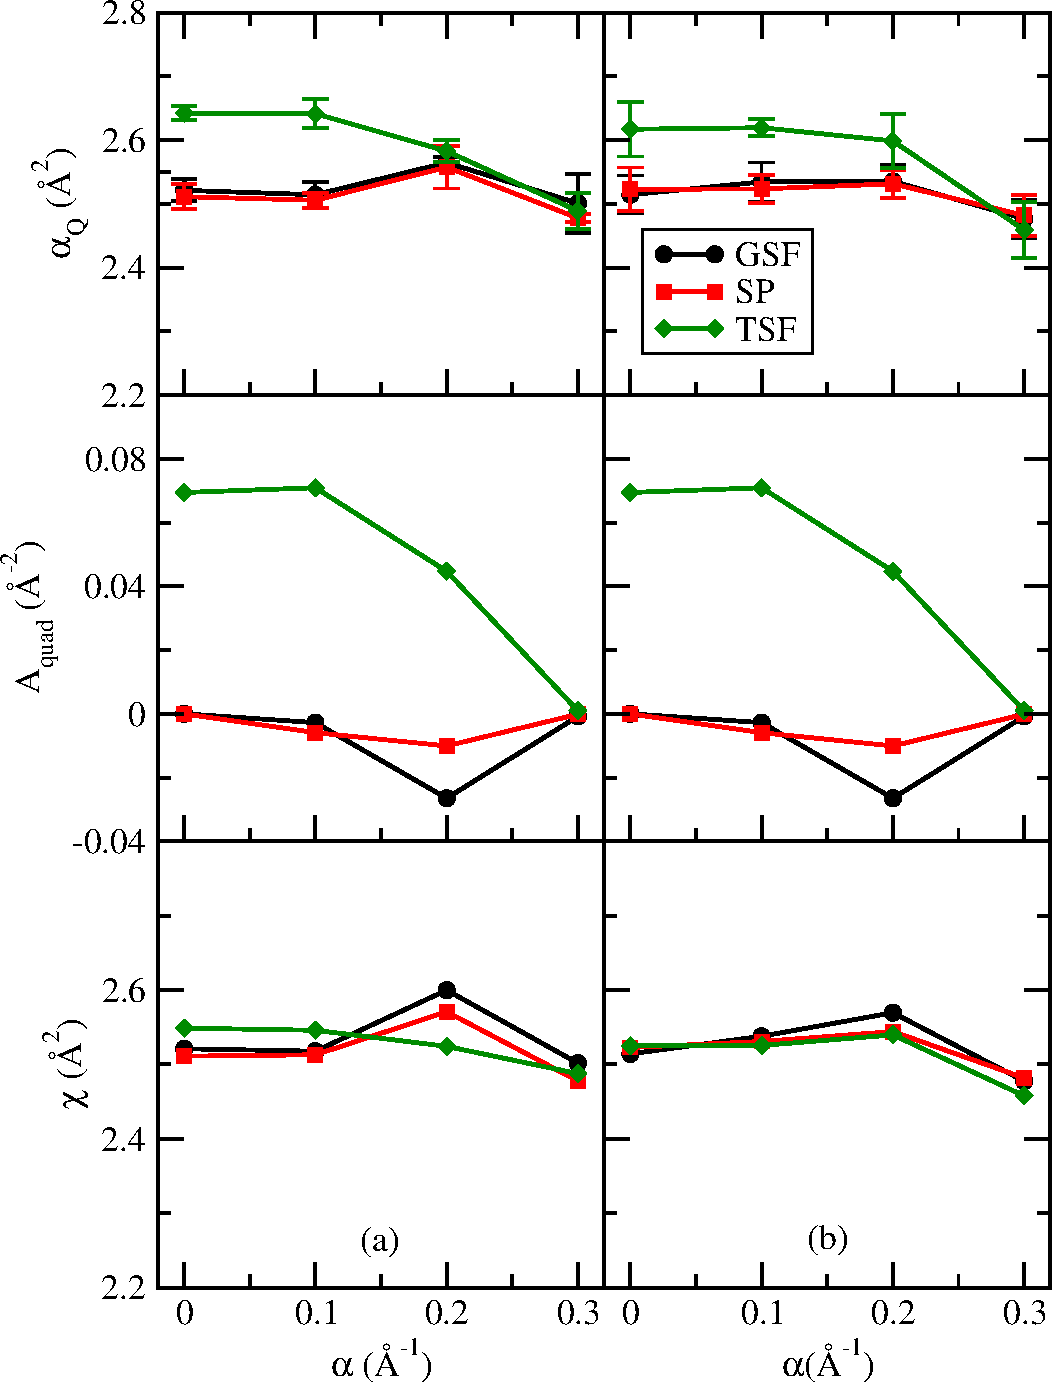
\includegraphics[width=\linewidth]{polarizabilityFinal_Quad.pdf}
\caption{In the figure, $\alpha_Q$, $\mathrm{A}_\mathrm{quad}$, and $\chi$  are polarizability, correction factor, and susceptibility for the quadrupolar fluid. Plots in the left panel show results for (a) perturbation method and right (b) fluctuation method.}
\label{fig:dielectricQuad}
\end{figure}

The actual test of the susceptibility can be made by comparing the results obtained from the perturbation and fluctuation with the result calculated from more direct, potential of mean force (PMF), method. For this purpose, we have calculated the expected dielectric constant from the susceptibility and geometrical factor using equation \ref{eq:dielectricFromQuadrupoles}. Since the dielectric constant for quadrupolar fluid is geometry-dependent, it is not a actual measure of the property of the quadrupolar fluid. This geometrical factor varies with the variation in ions separation as well as damping parameter therefore the dielectric constant can be refereed as screening factor. The screening factor plotted against ions separation, evaluated from the perturbation and fluctuation method are shown in right and central panel of the figure \ref{fig:screenQuad}. Here the susceptibility is calculated from the simulation and the geometrical factor is evaluated analytically, using field and field-gradient produced by ions. The right hand panel shows screening factor plotted against ions separation, for the different values of the damping alpha, obtained from the PMF method. The figure clearly shows that the screening factor obtained from the perturbation and fluctuation formula shows good agreement with the screening factor calculated using PMF method. Since there is no huge differences in quadrupole-quadruople interactions for various real-space methods, we do not observe large differences in the screen factors for SP, GSF, and TSF methods.        

\begin{figure}
  \centering
  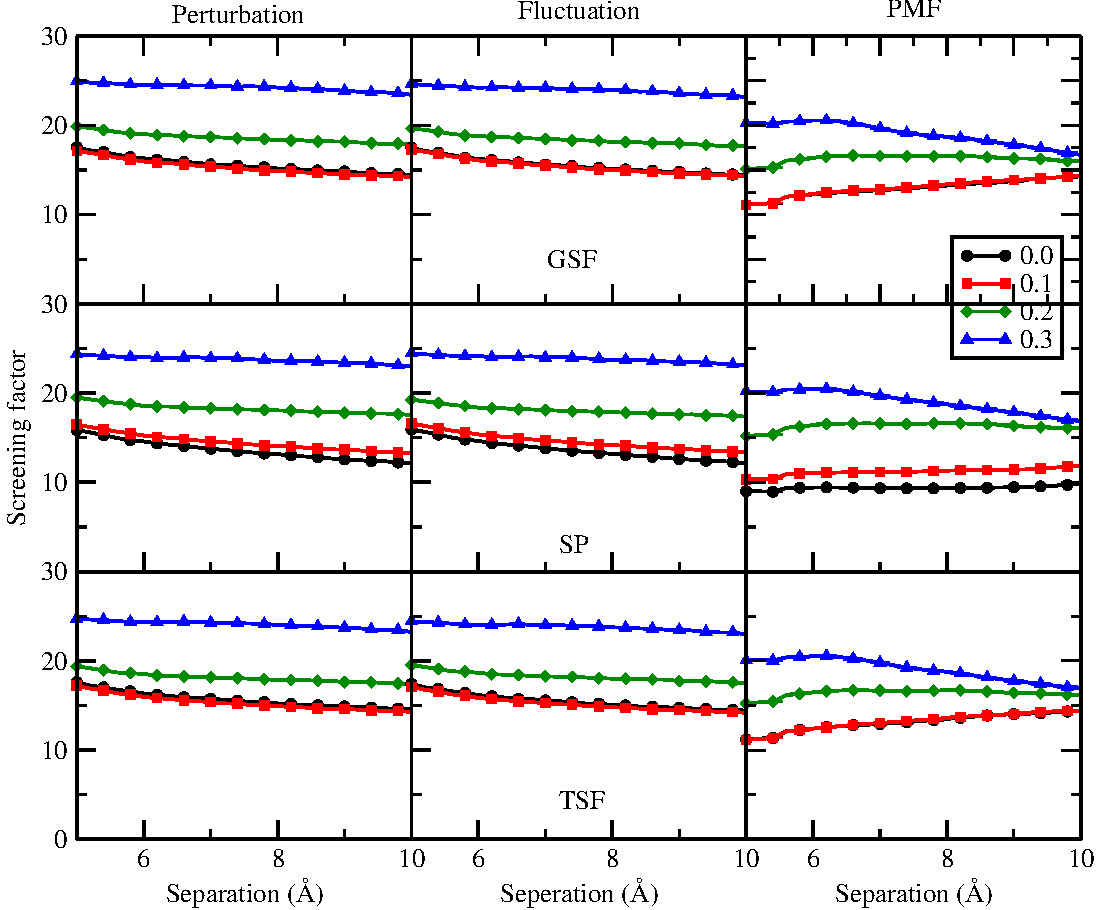
\includegraphics[width=\linewidth]{ScreeningFactor_Quad.pdf}
\caption{}
\label{fig:screenQuad}
\end{figure}

\section{Summary}
We have used the perturbation and fluctuation formula to evaluate dielectric properties for dipolar and quadrupolar fluids implementing SP, GSF, and TSF methods in the simulation. Similarly the correction factors for the both dipolar and quadrupolar systems have also been calculated for all SP, GSF, and TSF methods.  We have also derived screening factor between two ions immersed in the dipolar and quadrupolar fluids using PMF method. The result from the perturbation and fluctuation formula are compared with PMF method to test the accuracy of the simulation result. 

For the dipolar fluid, the polarizability evaluated using the perturbation and fluctuation methods show excellent agreement with each other. The dielectric constant evaluated using polarizability and correction factor agree with the previous simulation results \cite{NeumannI83} for the damping parameter 0.25 - 0.3$\AA^{-1}$ and the electrostatic interaction methods, SP and GSF implemented in the simulation. Since the correction factor for TSF, $\mathrm{A_{dipole}} = 1$, it produces dielectric constant more closer to previous simulation results \cite{NeumannI83} for all values damping parameter. This method also produces best dielectric constant for damping parameter 0.15 - 0.25$\AA^{-1}$. We have also found that correction formula (equation ~\ref{correctionFormula}) is very sensitive, when the correction factor ($\mathrm{A_{dipole}}$) much away from the 1 for the SP and GSF methods. Therefore it is better to choose damping parameter from 0.25 - 0.3$\AA^{-1}$ to evaluate dielectric constant using SP and GSF methods. The screening factor between ions is found to be closer to dielectric constant when the distance between the ions are far apart ($\sim 9 \AA$) and damping parameter $0.2$ to $0.3 \AA^{-1}$.

The quadpolarizability evaluated from the both perturbation and fluctuation methods shows excellent agreement with each other for the case of quadrupolar fluid. The susceptibility is calculated from the quadpolarizability and correction factor tends to produce same result for all; SP, GSF, and TSF, methods. Similarly the screening factor calculated using susceptibility and geometrical factor shows excellent agreement with the result obtained from the PMF method.

% % uncomment the following lines,
% if using chapter-wise bibliography
%
% \bibliographystyle{ndnatbib}
% \bibliography{example}
